\section{Cache}
	\subsection{Grundbegriffe}
		Der CPU Cache ist ein schneller Zwischenspeicher, der eine Teilmenge der Daten aus dem Arbeitsspeicher hält. Bei einem Arbeitsspeicherzugriff wird zuerst im Cache nachgeschaut, ob das angefragte Datum dort bereits existiert. Der Cache ist für den Programmierer in der Regel unsichtbar, er wird nicht direkt addressiert!
		\subsubsection{Cache Hit}
			Angefragtes Datum liegt bereits im Chache und kann daher deutlich schneller an das Registerwerk weitergeleitet werden
		\subsubsection{Cache Miss}
			Angefragtes Datum liegt nicht im Cache, muss daher aus dem Arbeitsspeicher geholt werden und wird anschließend im Cache abgelegt
	\subsection{Platzierung und Identifikation}
		\subsubsection{Cacheblöcke}
			Caches werden in sogenannte Blöcke gleicher Größe unterteilt. Beispielsweise könnte ein insgesamt 32 Byte großer Cache in 4 x 8 Byte große Blöcke unterteilt werden. Der Cache lädt dann bei einem Arbeitsspeicherzugriff immer 8 benachbarte Byte in einen Block.
			\newline \newline
			Die zu ladenden Nachbarn sind dabei immer auf die Cacheblockgröße \glqq aligned \grqq (vgl. Lernmodul 07): Das heißt, wenn wir zum Beispiel 8 Byte große Cacheblöcke haben, wird aus dem Arbeitsspeicher immer ein Nachbarpaket der Größe 8 Byte geholt, beginnend an einer Adresse, die Modulo 8 == 0 ist. 
			\newline \newline
			Das abgebildete Schaubild stellt das dar: Wir greifen auf das Byte der Adresse 0x19 (welches den Wert 0x30 hat) im Arbeitsspeicher zu, wodurch der ganze 8 Byte große Nachbarblock geladen wird. Die nähste, davor liegende Adresse, die Modulo 8 == 0 ist, ist die Adresse 0x18.
		\subsubsection{Byteoffset}
			Aus dieser Erkenntnis wissen wir, dass ein Teil der Arbeitsspeicheradresse immer die Funktion eines sogenannten Byteoffsets erfüllt. Wenn wir wie im ebigen Beispiel 8 Byte große Cacheblöcke haben, sind folglich die letzten 3 Bit (wegen $2^3=8$) der Arbeitsspeicheradresse das Byteoffset innerhalb eines Blockes. Um zum Beispiel aus dem 8 Byte großen Cacheblock die Zahl an der Adresse 0x19 (= 0001 1001) zu ziehen, müssten wir das 001'ste Byte (von links) nehmen.
		\subsubsection{Mengen / Index}
			Mehrere Cacheblöcke können zu einer Menge gruppiert werden. Innerhalb einer Menge dürfen wir zum Ablegen unserer Daten einen beliebigen Block wählen. Die Menge, in die wir die Daten legen, hängt wiederum von der Arbeitsspeicheradresse ab. Hierfür bestimmen wir den sogenannten Index
		\subsubsection{Tag}
			Der Tag sind die übrigen Bits einer Arbeitsspeicheradresse, die nicht für den Index oder das Byteoffset zuständig sind. Diese werden benötigt, um eine Adresse eindeutig rekonstruieren zu können und dadurch Konflikte zwischen ähnlichen Adressen zu vermeiden. Der Tag wird als "Metadaten" bei den Cacheblöcken gespeichert
			\newline
		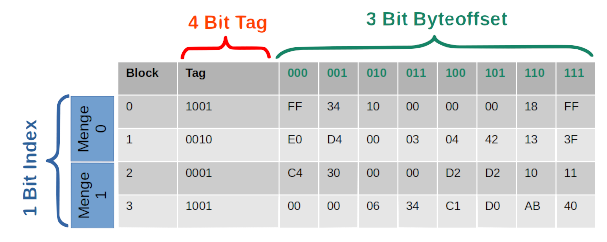
\includegraphics[scale=0.6]{tag.png}
	\subsection{Organisationsformen}
		\subsubsection{Vollassoziativ}
			 Ein Cache mit nur einer Menge, in welcher alle Blöcke sind. Wo man Datenblöcke ablegt ist also völlig beliebig und nicht anhand einer Adresse berechenbar.
		\subsubsection{Direktabbildend}
			Ein Cache mit Mengen, die jeweils aus genau einem Block bestehen. Man kann also 1:1 an der Arbeitsspeicheradresse (über den Index) "berechnen", in welcher Menge und dadurch auch welchem Block die Daten liegen.
		\subsubsection{N-fach assotiativ}
			Ein Cache mit Mengen, die aus jeweils n Blöcken bestehen. Hybridversion/Trade-Off zwischen den ersten beiden.
		\subsubsection{Vor und Nachteile} 
		\begin{itemize}
			\item Je mehr Blöcke pro Menge man hat, desto schwieriger ist es die Daten wieder zu finden
			\item Je weniger Blöcke pro Menge man hat, desto höher ist die Wahrscheinlichkeit, dass sich zwei Adressen gegenseitig verdrängen
		\end{itemize}
	\subsection{Ersetzungsstrategien}
			Innerhalb einer Menge (mit mindestens 2 Blöcken) können Daten in einen beliebigen Blöcke gelegt werden. Zu Beginn macht es Sinn, einfach einen freien Block zu nehmen. Wenn alle Blöcke voll sind, muss intelligent ein belegter Block ersetzt werden. Die eingesetzte Ersetzungsstrategie entscheidet, welcher Block für einen neuen verdrängt wird.
		\subsubsection{Random}
			Es wird "gewürfelt". (Nicht-vorhersagbares Cacheverhalten; dafür vergleichsweise leicht zu implementieren in Hardware)
		\subsubsection{LRU}
			Least Recently Used. Der Block, auf den am längsten nicht mehr zugegriffen wurde, wird verdrängt. (Liefert gute Hitraten in der Realität, aber ist schwer zu implementieren. Die Blöcke müssen sich ihre letzten Zugriffe merken, und man muss beim Verdrängen die Zeitstempel vergleichen/sortieren).
		\subsubsection{LFU}
			 Least Frequently Used. Der Block, auf den am seltensten zugegriffen wurde, wird verdrängt. (Ähnlich bzgl. Vor-/Nachteile wie LRU. Außerdem muss man beachten, dass es dadurch passieren kann, dass ein (zeitweise) häufig benutzter Block "für immer" im Cache bleibt, auch wenn er nun nicht mehr betrachtet wird. Der Counter muss am Besten periodisch wieder runtergesetzt werden)
		\subsubsection{FIFO} 
			First in, first out
	\subsection{Aktualisierungsstrategien}
		Die sogenannte Aktualisierungsstrategie eines Caches bestimmt, wie sich ein Cache verhält, wenn ein Datum geändert (aktualisiert) wird.
		\subsubsection{Write through}
			Alle Änderungen an Cacheinhalten werden direkt auch an die nächste Stufe der Speicherhierarchie (typischerweise der Arbeitsspeicher) weitergeleitet (durch den Cache durchgeschrieben). \newline
			\begin{itemize}
				\item Vorteil: Kohärenz zwischen Arbeitsspeicher und Caches (beide kennen immer die neusten Daten); insbesondere bei Mehrkernsystemen relevant.
				\item Nachteil: Sehr langsam, da ständig etwas an den Arbeitsspeicher geschickt wird. Blockiert dadurch die Arbeitsspeicherbandbreite.
			\end{itemize}
		\subsubsection{Write back}
			Änderungen an Cacheinhalten werden erst zurück in die nächste Stufe der Speicherhierarchie geschrieben, wenn der Cacheblock verdrängt wird. Um sich hier unnötiges Rückschreiben nicht-geänderter Daten zu sparen, wird sich bei jedem Block ein Dirty-Bit gemerkt. Dieses wird auf 1 gesetzt, wenn der Block aktualisiert wurde, was beim Verdrängen zum tatsächlichen Rückschreiben der Daten führt. Wenn es auf 0 bleibt, wird der Block einfach gelöscht und nicht zurückgeschrieben. \newline
			\begin{itemize}
				\item Vorteil: Wenn es viele Änderungen am Cacheblock gibt, wird es nur 1x am Ende zurückgeschrieben. Das spart Zeit/Performance
				\item Nachteil: Zeitweise große Inkonsistenz zwischen Cache und Arbeitsspeicher
			\end{itemize}


